% Options for packages loaded elsewhere
\PassOptionsToPackage{unicode}{hyperref}
\PassOptionsToPackage{hyphens}{url}
\PassOptionsToPackage{dvipsnames,svgnames,x11names}{xcolor}
%
\documentclass[
  letterpaper,
  DIV=11,
  numbers=noendperiod]{scrartcl}

\usepackage{amsmath,amssymb}
\usepackage{lmodern}
\usepackage{iftex}
\ifPDFTeX
  \usepackage[T1]{fontenc}
  \usepackage[utf8]{inputenc}
  \usepackage{textcomp} % provide euro and other symbols
\else % if luatex or xetex
  \usepackage{unicode-math}
  \defaultfontfeatures{Scale=MatchLowercase}
  \defaultfontfeatures[\rmfamily]{Ligatures=TeX,Scale=1}
\fi
% Use upquote if available, for straight quotes in verbatim environments
\IfFileExists{upquote.sty}{\usepackage{upquote}}{}
\IfFileExists{microtype.sty}{% use microtype if available
  \usepackage[]{microtype}
  \UseMicrotypeSet[protrusion]{basicmath} % disable protrusion for tt fonts
}{}
\makeatletter
\@ifundefined{KOMAClassName}{% if non-KOMA class
  \IfFileExists{parskip.sty}{%
    \usepackage{parskip}
  }{% else
    \setlength{\parindent}{0pt}
    \setlength{\parskip}{6pt plus 2pt minus 1pt}}
}{% if KOMA class
  \KOMAoptions{parskip=half}}
\makeatother
\usepackage{xcolor}
\setlength{\emergencystretch}{3em} % prevent overfull lines
\setcounter{secnumdepth}{-\maxdimen} % remove section numbering
% Make \paragraph and \subparagraph free-standing
\ifx\paragraph\undefined\else
  \let\oldparagraph\paragraph
  \renewcommand{\paragraph}[1]{\oldparagraph{#1}\mbox{}}
\fi
\ifx\subparagraph\undefined\else
  \let\oldsubparagraph\subparagraph
  \renewcommand{\subparagraph}[1]{\oldsubparagraph{#1}\mbox{}}
\fi


\providecommand{\tightlist}{%
  \setlength{\itemsep}{0pt}\setlength{\parskip}{0pt}}\usepackage{longtable,booktabs,array}
\usepackage{calc} % for calculating minipage widths
% Correct order of tables after \paragraph or \subparagraph
\usepackage{etoolbox}
\makeatletter
\patchcmd\longtable{\par}{\if@noskipsec\mbox{}\fi\par}{}{}
\makeatother
% Allow footnotes in longtable head/foot
\IfFileExists{footnotehyper.sty}{\usepackage{footnotehyper}}{\usepackage{footnote}}
\makesavenoteenv{longtable}
\usepackage{graphicx}
\makeatletter
\def\maxwidth{\ifdim\Gin@nat@width>\linewidth\linewidth\else\Gin@nat@width\fi}
\def\maxheight{\ifdim\Gin@nat@height>\textheight\textheight\else\Gin@nat@height\fi}
\makeatother
% Scale images if necessary, so that they will not overflow the page
% margins by default, and it is still possible to overwrite the defaults
% using explicit options in \includegraphics[width, height, ...]{}
\setkeys{Gin}{width=\maxwidth,height=\maxheight,keepaspectratio}
% Set default figure placement to htbp
\makeatletter
\def\fps@figure{htbp}
\makeatother

\usepackage{booktabs}
\usepackage{longtable}
\usepackage{array}
\usepackage{multirow}
\usepackage{wrapfig}
\usepackage{float}
\usepackage{colortbl}
\usepackage{pdflscape}
\usepackage{tabu}
\usepackage{threeparttable}
\usepackage{threeparttablex}
\usepackage[normalem]{ulem}
\usepackage{makecell}
\usepackage{xcolor}
\KOMAoption{captions}{tableheading}
\makeatletter
\makeatother
\makeatletter
\makeatother
\makeatletter
\@ifpackageloaded{caption}{}{\usepackage{caption}}
\AtBeginDocument{%
\ifdefined\contentsname
  \renewcommand*\contentsname{Table of contents}
\else
  \newcommand\contentsname{Table of contents}
\fi
\ifdefined\listfigurename
  \renewcommand*\listfigurename{List of Figures}
\else
  \newcommand\listfigurename{List of Figures}
\fi
\ifdefined\listtablename
  \renewcommand*\listtablename{List of Tables}
\else
  \newcommand\listtablename{List of Tables}
\fi
\ifdefined\figurename
  \renewcommand*\figurename{Figure}
\else
  \newcommand\figurename{Figure}
\fi
\ifdefined\tablename
  \renewcommand*\tablename{Table}
\else
  \newcommand\tablename{Table}
\fi
}
\@ifpackageloaded{float}{}{\usepackage{float}}
\floatstyle{ruled}
\@ifundefined{c@chapter}{\newfloat{codelisting}{h}{lop}}{\newfloat{codelisting}{h}{lop}[chapter]}
\floatname{codelisting}{Listing}
\newcommand*\listoflistings{\listof{codelisting}{List of Listings}}
\makeatother
\makeatletter
\@ifpackageloaded{caption}{}{\usepackage{caption}}
\@ifpackageloaded{subcaption}{}{\usepackage{subcaption}}
\makeatother
\makeatletter
\@ifpackageloaded{tcolorbox}{}{\usepackage[many]{tcolorbox}}
\makeatother
\makeatletter
\@ifundefined{shadecolor}{\definecolor{shadecolor}{rgb}{.97, .97, .97}}
\makeatother
\makeatletter
\makeatother
\ifLuaTeX
  \usepackage{selnolig}  % disable illegal ligatures
\fi
\IfFileExists{bookmark.sty}{\usepackage{bookmark}}{\usepackage{hyperref}}
\IfFileExists{xurl.sty}{\usepackage{xurl}}{} % add URL line breaks if available
\urlstyle{same} % disable monospaced font for URLs
\hypersetup{
  pdftitle={Analysis of Obesity Prevalence and Influencing Factors in the 2013--2016 Scottish Health Surveys},
  pdfauthor={Amina Rage (2652872R), Robin Purves (2763403P), Yassmine Boukhobezaa (2796790B), Yu Zhao (2724171Z)},
  colorlinks=true,
  linkcolor={blue},
  filecolor={Maroon},
  citecolor={Blue},
  urlcolor={Blue},
  pdfcreator={LaTeX via pandoc}}

\title{Analysis of Obesity Prevalence and Influencing Factors in the
2013--2016 Scottish Health Surveys}
\usepackage{etoolbox}
\makeatletter
\providecommand{\subtitle}[1]{% add subtitle to \maketitle
  \apptocmd{\@title}{\par {\large #1 \par}}{}{}
}
\makeatother
\subtitle{Group 6}
\author{Amina Rage (2652872R), Robin Purves (2763403P), Yassmine
Boukhobezaa (2796790B), Yu Zhao (2724171Z)}
\date{}

\begin{document}
\maketitle
\ifdefined\Shaded\renewenvironment{Shaded}{\begin{tcolorbox}[sharp corners, boxrule=0pt, breakable, enhanced, borderline west={3pt}{0pt}{shadecolor}, interior hidden, frame hidden]}{\end{tcolorbox}}\fi

\hypertarget{sec-intro}{%
\section{Introduction}\label{sec-intro}}

Obesity has become a significant public health concern in Scotland,
raising worries about the rising burden of chronic diseases and
healthcare costs. The 2013--2016 Scottish Health Surveys provide
valuable insights into socio-economic and lifestyle factors that may
influence obesity prevalence, including age, sex, education, and survey
year. This project seeks to determine whether the prevalence of obesity
has changed over time and to explore how demographic and socio-economic
factors relate to weight classification. By analyzing these trends, we
can gain a deeper understanding of the drivers behind obesity and inform
targeted public health interventions.

\hypertarget{sec-expdata}{%
\section{Exploratory data analysis}\label{sec-expdata}}

These statistics can be illustrated in Figure~\ref{fig-bar1} below. We
can also see that there are no significant change in the proportion of
obese individuals between 2013 and 2016.

\begin{figure}

{\centering 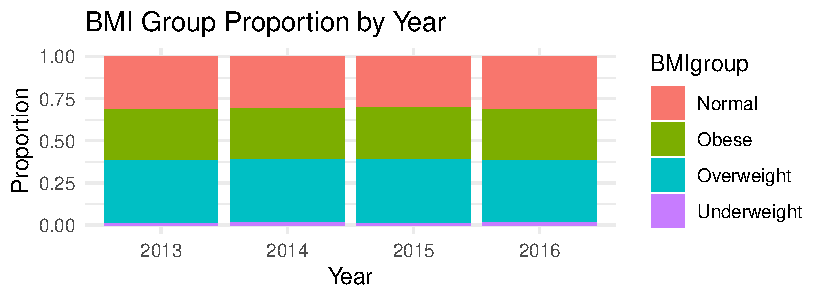
\includegraphics{Data-analysis-12-main_files/figure-pdf/fig-bar1-1.pdf}

}

\caption{\label{fig-bar1}bar plot of BMIgroup by year}

\end{figure}

Next, we want to explore the relationship between Age and BMIgroup.In
Figure~\ref{fig-box1} shows that the age distribution varies
significantly across different BMI groups. Generally, obese individuals
tend to be older, whereas the underweight group is comparatively
younger. This indicates age is an important factor associated with BMI
categories.

\begin{figure}

{\centering 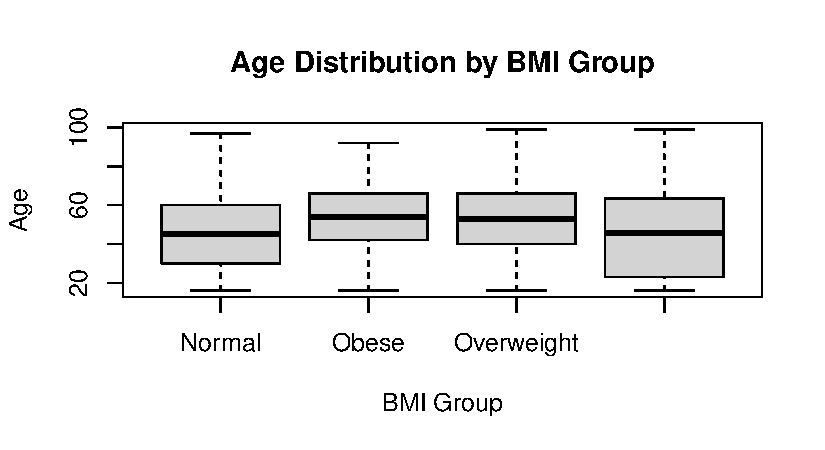
\includegraphics{Data-analysis-12-main_files/figure-pdf/fig-box1-1.pdf}

}

\caption{\label{fig-box1}Box plot showing the relationship between Age
and BMIgroup}

\end{figure}

Next, we analyse the relationship between BMI Group Proportion by Sex.
In Figure~\ref{fig-bar2} we see there are noticeable differences in BMI
group proportions between males and females. Males appear slightly more
likely to be overweight, whereas females show relatively higher
proportions in the normal and obese categories. Gender thus influences
BMI distribution patterns.

\begin{figure}

{\centering 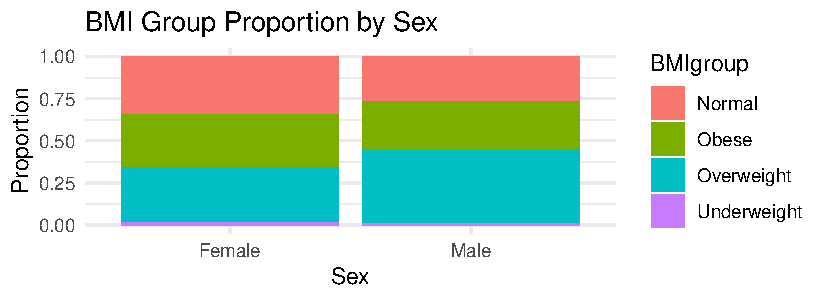
\includegraphics{Data-analysis-12-main_files/figure-pdf/fig-bar2-1.pdf}

}

\caption{\label{fig-bar2}Bar plot showing the relationship between Sex
and BMIgroup}

\end{figure}

Finally, we want to assess the relationship between Education and
BMIgroup. In Figure~\ref{fig-bar3} shows that the education level is
related to BMI groups. Individuals with higher educational
qualifications generally have higher proportions of normal weight and
lower proportions of obesity. Conversely, individuals with fewer or no
qualifications show a greater proportion of obesity. Socio-economic
factors, represented by education levels, clearly impact obesity rates.

\begin{figure}

{\centering 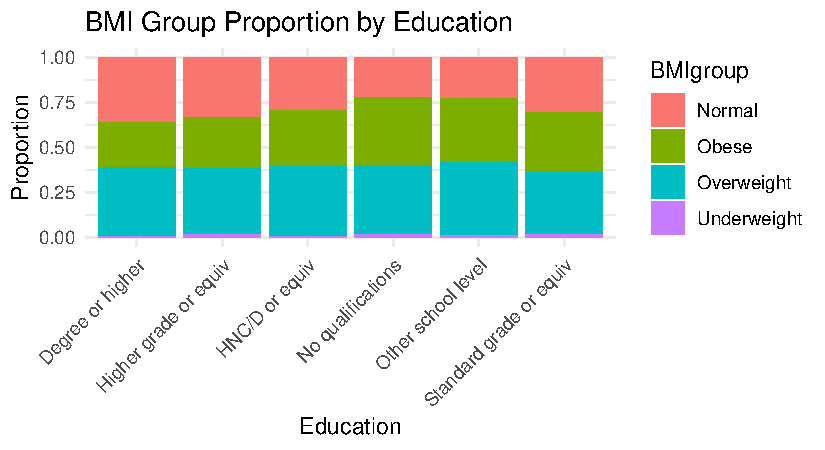
\includegraphics{Data-analysis-12-main_files/figure-pdf/fig-bar3-1.pdf}

}

\caption{\label{fig-bar3}Bar plot showing the relationship between
Education and BMIgroup}

\end{figure}

\hypertarget{sec-formdata}{%
\section{Formal data analysis}\label{sec-formdata}}

\begin{verbatim}

    Chi-squared Test for Trend in Proportions

data:  trend_table[, 2] out of rowSums(trend_table) ,
 using scores: 1 2 3 4
X-squared = 0.11404, df = 1, p-value = 0.7356
\end{verbatim}

\begin{verbatim}
[1] 2016 2015 2014 2013
\end{verbatim}

\begin{verbatim}
[1] 1 0
\end{verbatim}

\begin{verbatim}

    Pearson's Chi-squared test

data:  trend_table
X-squared = 0.22577, df = 3, p-value = 0.9733
\end{verbatim}

\begin{longtable}[]{@{}cccc@{}}
\toprule()
~ &
\multicolumn{3}{>{\centering\arraybackslash}p{(\columnwidth - 6\tabcolsep) * \real{0.0000} + 4\tabcolsep}@{}}{%
obese binary} \\
\midrule()
\endhead
Predictors & Odds Ratios & CI & p \\
(Intercept) & 0.43 & 0.39~--~0.47 & \textbf{\textless0.001} \\
Year & 1.01 & 0.97~--~1.04 & 0.736 \\
\bottomrule()
\end{longtable}

The formal analysis of obesity prevalence trends in Scotland, using data
from the Scottish Health Survey, reveals no statistically significant
change over the surveyed years (2013--2016). The Chi-squared Test for
Trend in Proportions (X²=0.114, p=0.736) and Pearson's Chi-squared Test
(X²=0.226, p=0.973) both fail to reject the null hypothesis, indicating
no evidence of a linear trend or overall difference in obesity
proportions across the years. This conclusion is further supported by
the logistic regression results, where the ``Year'' variable shows an
odds ratio of 1.01 (95\% CI: 0.97--1.04, p=0.736), suggesting that each
passing year was associated with a non-significant change in obesity
odds. The intercept (OR=0.43, p\textless0.001) reflects the baseline
odds of obesity but does not inform temporal trends. Overall, these
results demonstrate that obesity prevalence in Scotland remained stable
during the study period, with no meaningful increase or decrease
detected.

\hypertarget{question-2}{%
\subsubsection{Question 2}\label{question-2}}

To answer the second question, we use linear regression to find out if
age, gender, socio-economic status, or lifestyle factors are significant
predictors for obesity.

We start by looking at if age is a significant predictor for a persons
BMI group. We are fitting the following linear model:

\[
logit(\pi) = \beta_0 + \beta_1 x_i + \epsilon_i, ~~~~~ \epsilon_i \sim N(0, \sigma^2), ~~~~~ i = 1, ... , 14017
\]

Here, \(\pi\) is the probability that the individual is obese, \(x_i\)
is the age of the ith individual, and \(\beta_0\), \(\beta_1\) are
regression coefficients. We are using the logit link function.

\begin{longtable}[]{@{}cccc@{}}
\toprule()
~ &
\multicolumn{3}{>{\centering\arraybackslash}p{(\columnwidth - 6\tabcolsep) * \real{0.0000} + 4\tabcolsep}@{}}{%
BM Igroup} \\
\midrule()
\endhead
Predictors & Odds Ratios & CI & p \\
(Intercept) & 4.33 & 3.86~--~4.86 & \textbf{\textless0.001} \\
Age & 0.99 & 0.99~--~0.99 & \textbf{\textless0.001} \\
\bottomrule()
\end{longtable}

As seen from the p-value, we can infer that age is a significant
predictor for a persons BMI group. As someones age increases by one
year, the odds of the person being obese increase by a factor of 0.99.

We now check the assumptions of our model, to find out if the model is
valid.

\begin{figure}

{\centering 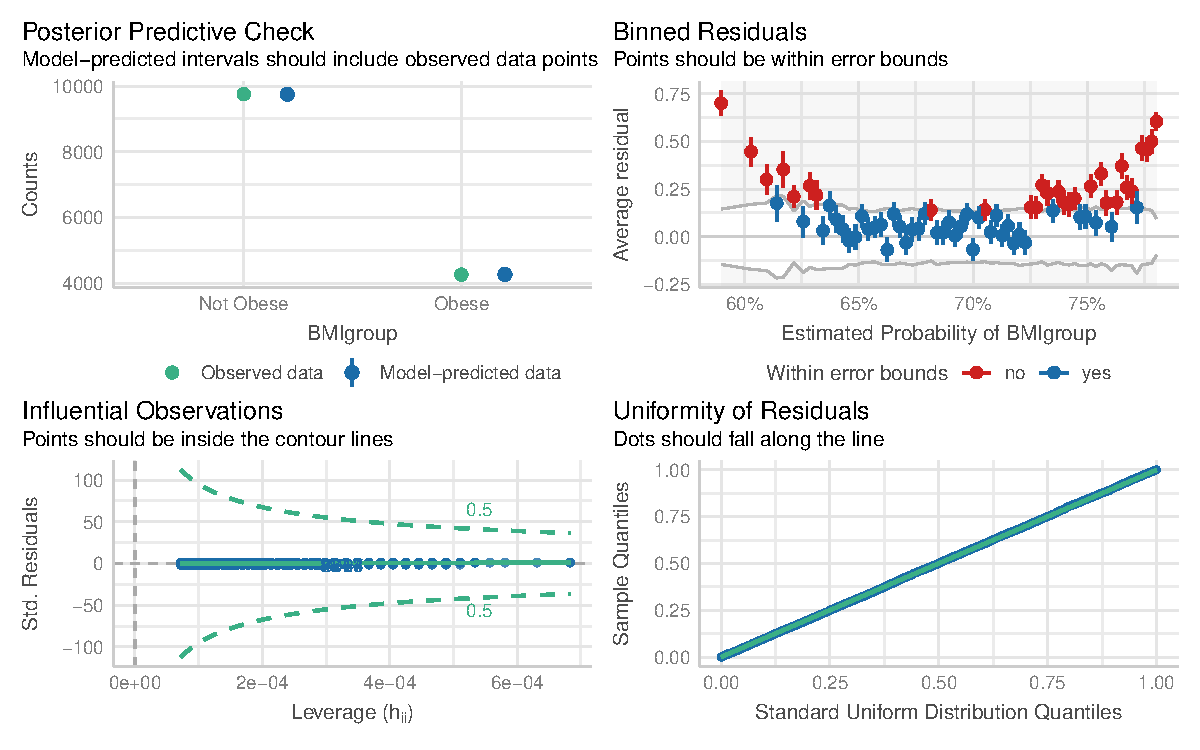
\includegraphics{Data-analysis-12-main_files/figure-pdf/fig-diagnostics1-1.pdf}

}

\caption{\label{fig-diagnostics1}Diagnostic plots for the age model}

\end{figure}

There is no issues that can be seen in the posterior predictive check,
influential observations graph, and the uniformity of residuals graph.
There does appear to be a large amount of points falling outside the
error bounds in the binned residuals graph. We would expect about 95\%
of points to fall within the error bounds if the model is true. As there
is a large amount of points plotted it is hard to tell if there is 95\%
within the error bounds, as there may be overlap. However, it appears to
be good enough.

We now look at sex to consider if it is significant through fitting the
following model:

\[
logit(\pi) = \beta_0 + \beta_1 x_i + \epsilon_i, ~~~~~ \epsilon_i \sim N(0, \sigma^2), ~~~~~ i = 1, ... , 14017
\]

Where \(x_i\) is an indicator variable taking the value 0 if the
individual is a male and the value 1 if the individual is a female.

\begin{longtable}[]{@{}cccc@{}}
\toprule()
~ &
\multicolumn{3}{>{\centering\arraybackslash}p{(\columnwidth - 6\tabcolsep) * \real{0.0000} + 4\tabcolsep}@{}}{%
BM Igroup} \\
\midrule()
\endhead
Predictors & Odds Ratios & CI & p \\
(Intercept) & 2.44 & 2.31~--~2.57 & \textbf{\textless0.001} \\
Sex {[}Female{]} & 0.89 & 0.83~--~0.96 & \textbf{0.002} \\
\bottomrule()
\end{longtable}

As seen from table 2, the p-value indicates that sex is a significant
predictor at the 5\% significance level. Furthermore, the odds ratio for
being obese increase by 0.89 for females.

Again, we check our model assumptions to find out if our results are
valid.

\begin{figure}

{\centering 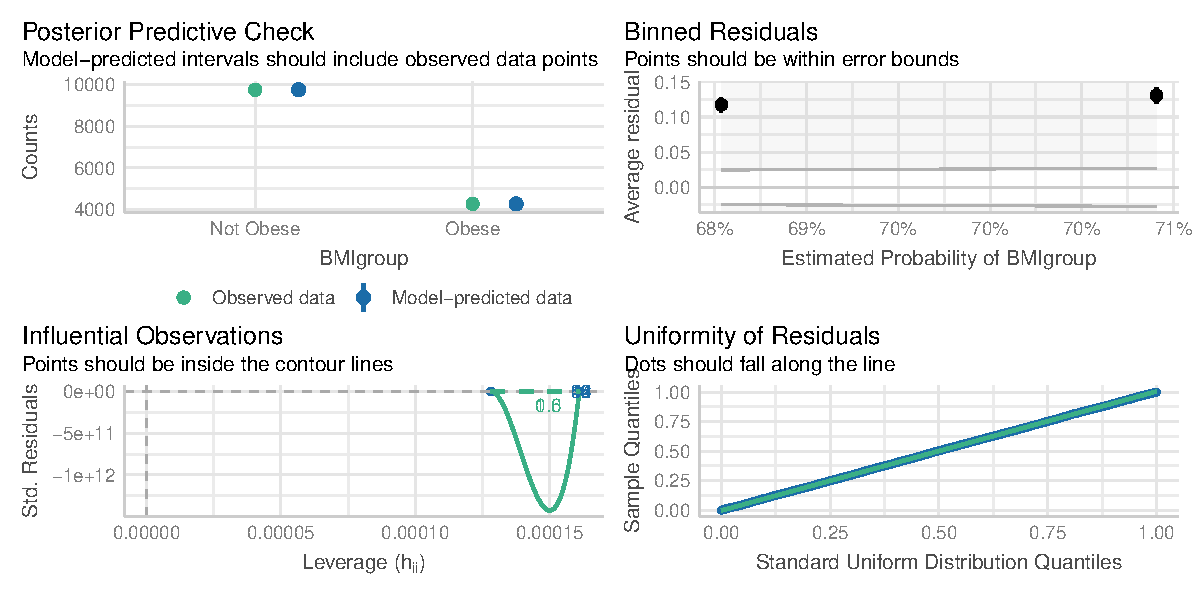
\includegraphics{Data-analysis-12-main_files/figure-pdf/fig-diagnostics2-1.pdf}

}

\caption{\label{fig-diagnostics2}Diagnostic plots for the sex model}

\end{figure}

The plots in figure 2 look good enough. There may be issues with the
binned residuals plot, however the issue likely stems from sex being a
factor with 2 levels giving us only 2 points.

We now look at education to consider if there is a difference in obesity
based on socio-economic factors. We fit the following model:

\[
logit(\pi) = \beta_0 + \beta_1 x_i + \beta_2 x_j + \beta_3 x_k + \beta_4 x_l +\beta_5 x_m + \beta_6 x_n + \epsilon_i, ~~~~~ \epsilon_i \sim N(0, \sigma^2), ~~~~~ i = 1, ... , 14017
\] Where \(x_i\) through \(x_n\) are indicator variables taking the
value 1 if they have that level of education and 0 if they do not. The
\(\beta_0\) term refers to the reference level which is having a degree.

\begin{longtable}[]{@{}
  >{\centering\arraybackslash}p{(\columnwidth - 6\tabcolsep) * \real{0.2500}}
  >{\centering\arraybackslash}p{(\columnwidth - 6\tabcolsep) * \real{0.2500}}
  >{\centering\arraybackslash}p{(\columnwidth - 6\tabcolsep) * \real{0.2500}}
  >{\centering\arraybackslash}p{(\columnwidth - 6\tabcolsep) * \real{0.2500}}@{}}
\toprule()
\begin{minipage}[b]{\linewidth}\centering
~
\end{minipage} &
\multicolumn{3}{>{\centering\arraybackslash}p{(\columnwidth - 6\tabcolsep) * \real{0.7500} + 4\tabcolsep}@{}}{%
\begin{minipage}[b]{\linewidth}\centering
BM Igroup
\end{minipage}} \\
\midrule()
\endhead
Predictors & Odds Ratios & CI & p \\
(Intercept) & 3.05 & 2.85~--~3.26 & \textbf{\textless0.001} \\
\begin{minipage}[t]{\linewidth}\raggedright
Education {[}Higher grade\\
or equiv{]}\strut
\end{minipage} & 0.84 & 0.75~--~0.94 & \textbf{0.003} \\
\begin{minipage}[t]{\linewidth}\raggedright
Education {[}HNC/D or\\
equiv{]}\strut
\end{minipage} & 0.72 & 0.64~--~0.82 & \textbf{\textless0.001} \\
\begin{minipage}[t]{\linewidth}\raggedright
Education {[}No\\
qualifications{]}\strut
\end{minipage} & 0.53 & 0.48~--~0.59 & \textbf{\textless0.001} \\
\begin{minipage}[t]{\linewidth}\raggedright
Education {[}Other school\\
level{]}\strut
\end{minipage} & 0.60 & 0.51~--~0.70 & \textbf{\textless0.001} \\
\begin{minipage}[t]{\linewidth}\raggedright
Education {[}Standard grade\\
or equiv{]}\strut
\end{minipage} & 0.67 & 0.60~--~0.74 & \textbf{\textless0.001} \\
\bottomrule()
\end{longtable}

As seen from table 3, all the levels of education are considered
significant predictors of the persons BMI group. The odds of a person
being obese is 3.05 for a person with a degree, then increases by
0.53-0.84 depending on qualification level.

Again, we have to check the model assumptions.

\begin{figure}

{\centering 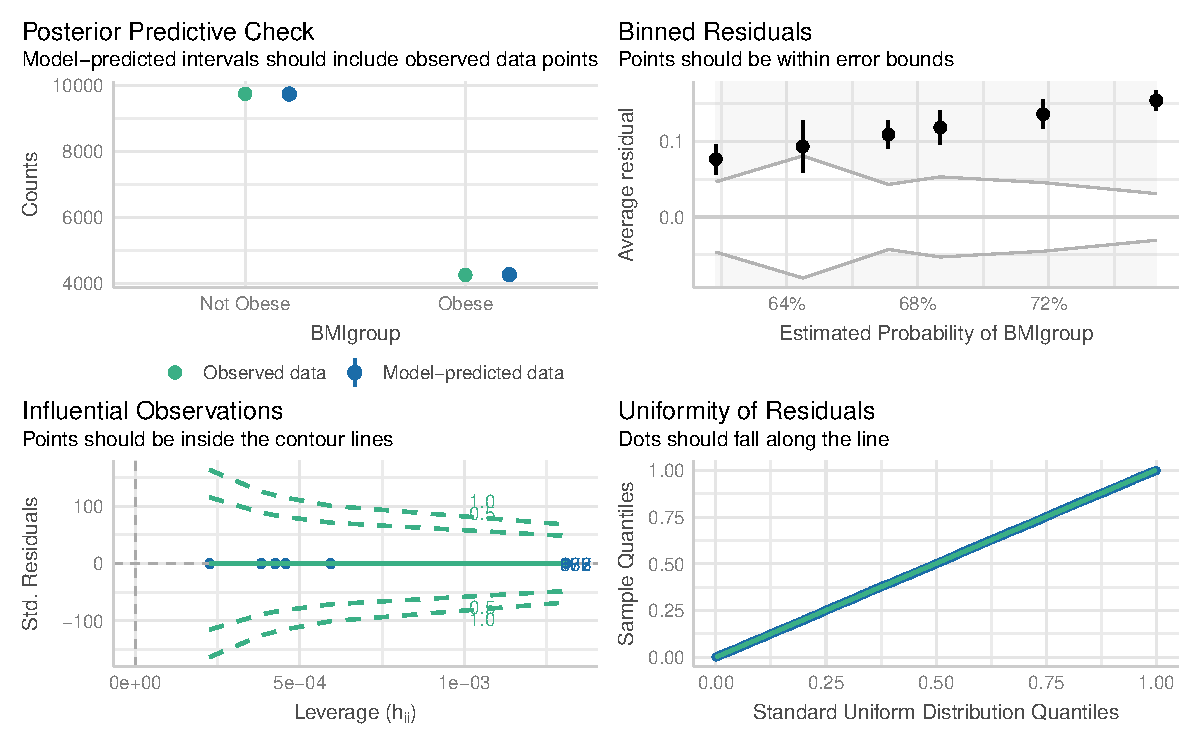
\includegraphics{Data-analysis-12-main_files/figure-pdf/fig-diagnostics3-1.pdf}

}

\caption{\label{fig-diagnostics3}Diagnostic plots for the education
model}

\end{figure}

The interpretation of figure 3 is much like the previous figures. The
only graph that leaves cause for concern is the binned residuals graph,
but again, because it is a factor, it is always going to not work as
well as a continuous variable. Thus, the model is appropriate.

\hypertarget{sec-conc}{%
\section{Conclusions}\label{sec-conc}}

The analysis of the Scottish Health Survey data suggests that there has
been no significant change in obesity prevalence in Scotland between
2013 and 2016, as indicated by the stable proportion of BMI groups over
time.Furthermore, demographic and socio-economic factors appear to play
a role in obesity distribution:

\begin{itemize}
\item
  Older individuals are more likely to be classified as obese, while
  younger individuals are more frequently found in the underweight
  category
\item
  Males tend to have a higher proportion of overweight individuals,
  whereas females exhibit relatively greater proportions in the normal
  and obese BMI categories.
\item
  Higher educational qualifications are associated with a lower
  prevalence of obesity, whereas individuals with fewer or no
  qualifications tend to have a higher proportion of obesity.
\end{itemize}

These findings suggest that while overall obesity rates have remained
stable, socio-demographic factors such as age, gender, and education
level significantly influence obesity.



\end{document}
